\documentclass{beamer}
\usepackage{graphicx} % Required for inserting images
\usepackage{subcaption}
\usepackage{booktabs}
\usepackage{chngcntr} 
\usepackage{comment}
\usepackage{mathtools}
\usepackage{color}
\usepackage{amssymb}
\usepackage{physics}
\usepackage{xurl}
\usepackage{siunitx}
\usepackage{float}
\usepackage{stmaryrd}
\usepackage[backend=biber, style=authortitle, sorting=none]{biblatex}
\addbibresource{references.bib}
\usetheme{Berlin}
\title{Dimensional Reduction in Supergravity and Duality Symmetries}
\author{Adam Franchot--Fowler}
\institute{University Paris-Saclay and ENS Lyon}
\usepackage{tcolorbox}
\tcbuselibrary{skins}

\usepackage{tcolorbox}
\tcbuselibrary{skins}

\newtcolorbox{eqbox}{
    colback=structure!10,
    colframe=structure,
    arc=3mm,
    boxrule=1pt,
}
\begin{document}

\begin{frame}
\titlepage
\end{frame}

\begin{frame}
\frametitle{Overview}
\tableofcontents
\end{frame}

\section{Introduction}
\begin{frame}
\begin{columns}
\column{0.5\textwidth}
\centering\textbf{Other force}\\
quantum field-theoretic language
\vspace{20mm}\pause
\column{0.5\textwidth}
\centering\textbf{General relativity}\\
Gravitational interaction due to space time deformation\\
\centering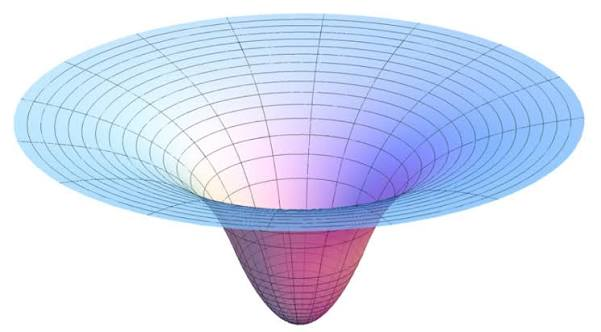
\includegraphics[width=0.5\textwidth]{images.jpg}
\end{columns}
\vspace{(5mm)}\pause
\centering{The classical quanfication method do not work on gravity. We need to modify the gravity description.}
\end{frame}
\begin{frame}
    \centering\textbf{supersymmetry}\\
    \centering{symmetry mixing the degrees of
freedom of fermions and bosons.\\
Used in :}
\vspace{15mm}
\begin{columns}
    \column{0.5\textwidth}
    \centering\boxed{\textbf{Supergravity}}\\
    \centering
\includegraphics[width=0.6\textwidth]{images2.jpg}
    \column{0.5\textwidth}
    \centering\boxed{\textbf{String Theory}}\\
    \centering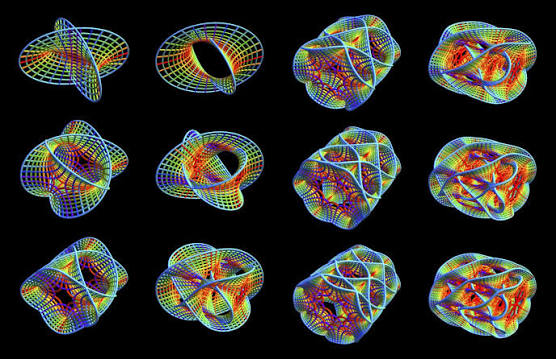
\includegraphics[width=0.5\textwidth]{images3.jpg}
\end{columns}
\vspace{10mm}\pause
\centering{!!\textbf{Both theories describe the existence of extra dimensions}!!}
\end{frame}
\begin{frame}
\centering{We need a way to describe how $4$ dimensions observer, see a $4+E$ dimensions universe.}\\
\vspace{5mm}
\centering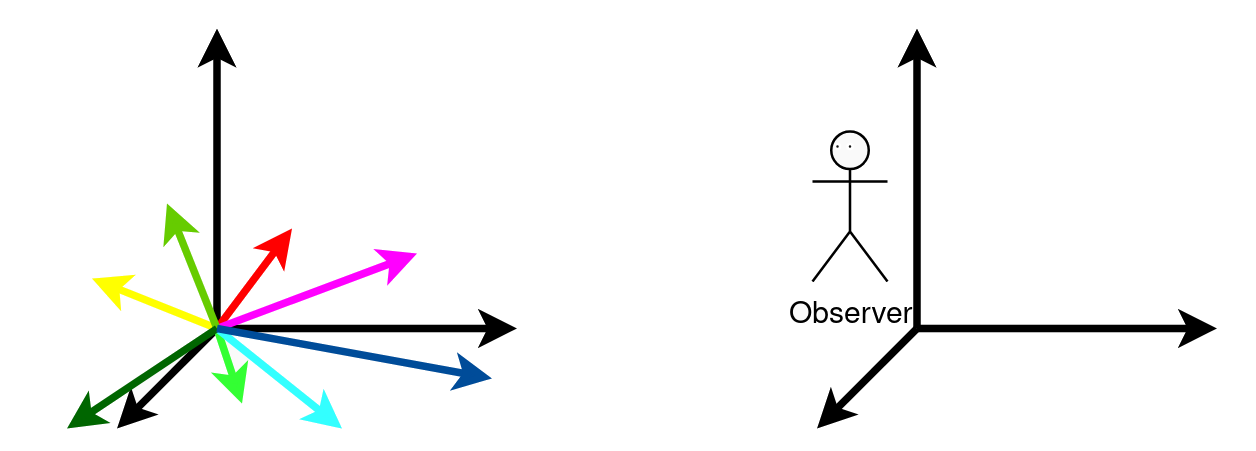
\includegraphics[width=0.8\textwidth]{images4.png}
\end{frame}
\section{$D+E$ gravity description}

   

\begin{frame}{$4$ dimension gravity}
    \begin{itemize}
     \item We describe GR as a deformation of space-time describe in a metric:
    \begin{equation*}
        g_{\mu \nu} = \begin{pmatrix}
            g_{00} & g_{01} & g_{02} & g_{03} \\
            g_{01} & g_{11} & g_{12} & g_{13} \\
            g_{02} & g_{12} & g_{22} & g_{23}\\
            g_{03} & g_{13} & g_{23} & g_{33}  
        \end{pmatrix}
    \end{equation*} \pause
    \item Einstein eqation: $R_{\mu \nu} \frac{1}{2}g_{\mu \nu}R = 0$.\pause \\
   This give us the hilbert-Einstein action :
    \begin{equation*}
      \boxed{  S_{g} = \int dx^4 \sqrt{-g} R}
    \end{equation*}
\end{itemize}
\end{frame}
\begin{frame}{electromagnetic $4$ dimensions description}
    \begin{columns}
        \column{0.4\textwidth}
        \centering{\textbf{Maxwell equations}}
        \begin{itemize}
            \item $\vec{\nabla} \cdot \vec{E} = \mu_0 c^2 \rho$,
            \item $\vec{\nabla} \times \vec{B} = \mu_0 \vec{j} + \frac{1}{c^2} \pdv{\vec{E}}{t}$,
            \item $\vec{ \nabla} \times - \pdv{\vec{B}}{t}$,
            \item $\vec{\nabla} \cdot \vec{B} = 0$.
        \end{itemize}
        \column{0.6\textwidth}\pause
        \centering{\textbf{Covariant formulation}}
        \begin{itemize}
        \item Four-current: $J^\mu = (c \rho , \vec{j})$, \\
        \item Four-potential: $A^\mu = (V/c, \vec{A})$,
        \item field strength: $F_{\mu \nu} = \partial_\mu A_\nu - \partial_\nu A_\mu$.\\
        \end{itemize}
        \vspace{6mm}\pause
    \end{columns}
    \vspace{10mm}
This give us the electromagnetic action or Maxwell action in a vaccum:
\begin{equation*}
    \boxed{S_{F} = \int dx^4 \frac{1}{4} F_{\mu \nu}F^{\mu \nu}}
\end{equation*}
\end{frame}
\begin{frame}{$D+E$ dimensions metric}
    If we add new dimension the action have to be modified:\\
    \begin{equation*}
         S_{\hat g} =\int d x^{D} \int \frac{d y ^E}{\rho(E)} \sqrt{- \hat g} \hat  R
    \end{equation*}\pause
    and the action will have to be expended, for example in $5$ dimension we have:
    \begin{equation*}
           \hat g_{\mu \nu} = \begin{pmatrix}
            g_{00} & g_{01} & g_{02} & g_{03}& g_{04} \\
            g_{01} & g_{11} & g_{12} & g_{13} & g_{14}\\
            g_{02} & g_{12} & g_{22} & g_{23}& g_{24}\\
            g_{03} & g_{13} & g_{23} & g_{33}  & g_{34} \\
            g_{04} & g_{14} & g_{24} & g_{34} & g_{44}
        \end{pmatrix}
    \end{equation*}
\end{frame}
\begin{frame}{Reduction}
    We are going to follow the reduction method of the \cite{scherk1979get}. Firstly let's do an anstaz of the metric we are going to use
    \begin{equation*}
         \hat g_{\hat \mu \hat \nu} = \begin{pmatrix}
        g_{\mu \nu} - A^{\gamma}_{\mu}A^{(1)}_{\nu \lambda} & - A^{(1)}_{\mu \beta} \\  A^{(1)}_{\nu \alpha} &-h_{\alpha \beta} \end{pmatrix}
    \end{equation*}\pause
    And once finished that gave us:
   \begin{equation*}
    \boxed{
    \begin{aligned}
    S_{\hat g} = &\int d x^D e^{-\hat \phi} V \delta \Big( 
    \frac{-1}{4} g^{\rho \lambda} \partial_\lambda h_{\alpha \beta}\partial_\rho h^{\alpha \beta}
    +\frac{1}{4}F^{\mu \nu \alpha}F^{\beta}_{\mu  \nu}h_{\alpha \beta}+\\
    &+ R + \frac{1}{4} \partial_{\hat \mu} \log(h) \partial^{\hat \mu} \log(h) + \partial_{\hat \mu} \log(h) \partial^{\hat \mu} \hat \phi \Big).
\end{aligned}}
\end{equation*}
\end{frame}
\section{$O(E,E)$ symmetry}
\begin{frame}{The NS-NS action}
    In string theory we do not use the Einstein Hilbert action but a variant of it the NS-NS action:
    \begin{equation*} 
    \boxed{S = \int d x^{D} \int \frac{d y^E}{\rho(E)}\sqrt{- \hat g } e^{ - \hat \phi} \Big(\hat R +  \partial_{\hat \mu}\hat \phi \partial^{\hat \mu}\hat \phi - \frac{1}{12}  H_{ \mu \nu \rho}H^{ \mu\nu \rho}\Big),}
\end{equation*} \pause
$\hat \phi$ is the dilaton, and $\hat H_{\hat \mu \hat \nu \hat \rho}$ is the srength field of the two form $ \hat B_{\mu \nu}$.We define the low components of  $ \hat B_{\mu \nu}$ with:
\begin{subequations} 
    \begin{align}
        T^{\mu} &= V_r^\mu \hat V^r_{\hat \mu}\hat T^{\hat \mu}, \\ 
        T^{\alpha} &= V_a^\alpha \hat V^a_{\hat \mu}\hat T^{\hat \mu}, \\ 
        T_{\mu} &= V_\mu^r \hat V_r^{\hat \mu}\hat T_{\hat \mu},\\  
        T_{\alpha} &= V_\alpha^a \hat V_a^{\hat \mu}\hat T_{\hat \mu}.  
    \end{align}
\end{subequations}
\end{frame}
\begin{frame}{An action reformed}
    We can now write the Reduced action :
    \begin{equation*}
        \boxed{
    \begin{aligned}
    S = &\int dx^D Ve^{-\phi}\Big( R +\partial_{\mu }\phi \partial^{\mu} \phi + \frac{1}{8}\tr(\partial_\mu M^{-1}\partial^\mu M)\\ 
    & -\frac{1}{4} \mathcal{F}^i_{\mu \nu}(M^{-1})_{ij} \mathcal{F}^{\mu \nu j}-\frac{1}{12}H_{\mu \nu \rho} H^{\mu \nu \rho} \Big).
    \end{aligned}}
\end{equation*}
with M being:
\begin{equation*}
     M = \begin{pmatrix}
        h^{-1} & -h^{-1}B \\ Bh^{-1} & h-Bh^{-1}B
    \end{pmatrix}.
\end{equation*}
\end{frame}
\begin{frame}{$O(E,E)$ invariance}
    We define the action of the $O(E,E)$ group as being, 
    \begin{align*} 
    &A^i \rightarrow \Omega^i_j A^j, \\
    &M_{ij} \rightarrow \Omega^l_i M_{lk}\Omega^k_j,
\end{align*}
where $\Omega \in O(E,E)$. \\
\centering{\textbf{The action is invariant under this transformation !!!!}}
\end{frame}
\section{Conclusion}
\begin{frame}{physical interpretation}
\begin{itemize}
    \item coupling of gravity and elctrmagnetism in low dimension from gravity in high dimension
    \item The NS-Ns action is $O(E,E)$ invariant.
\end{itemize}
\end{frame}
\begin{frame}{prospect}
    \begin{itemize}
        \item searching other symmetry
        \item considering an internal field dependence.
    \end{itemize}
\end{frame}
\section{annex}
\begin{frame}
     A matrix $M$ is in $O(E,E)$ if it is a square $E\times E$ matrix and, for the matrix
    \begin{equation*}
        \zeta = \begin{pmatrix}
            0 & 1 \\ 1 &0
        \end{pmatrix},
    \end{equation*}
    which can be used as a metric for the group $O(E,E)$, as it has $E$ negative eigenvalues and $E$ positive eigenvalues in a basis rotated from the one with diagonal metric,\\ 
    the matrix $M$ satisfies
    \begin{equation*}
        \boxed{M^T \zeta M = \zeta. }
    \end{equation*}
\end{frame}
\end{document}